\section{CHSH-Ungleichung}
\label{sec:chsh}


\subsection{Geschichte}
\label{subsec:chsh_geschichte}
Die CHSH-Ungleichung ist ein Beweis der Bell-Ungleichungen, die aus der Diskussion entstanden sind, ob die Quantenmechanik eine Theorie ist,
die die Realität vollständig abbildet.\ Diese Diskussion an sich ist Bestandteil einer weiteren Diskussion zwischen Niels Bohr und Albert einstein,
die als Bohr-Einstein Debatte bekannt ist, auf die hier nicht im Detail eingegangen wird.\ Der Beginn des Diskussionsteils, auf den wir uns fokussieren,
ist die Veröffentlichung des nach den Autoren benannten EPR-Paradoxons von Albert Einstein, Boris Podolsky und Nathan Rosen.\\
In dem Paper ''Can Quantum-Mechanical Description of Physical Reality Be Considered Complete?'' argumentieren Einstein, Podolsky und Rosen, dass
eine Theorie nur dann vollständig sein kann, wenn es zu jedem Element der physischen Realität ein Element in der Theorie geben müsse, was das Element
der physischen Realität abbilde/beschreibe.\ Als 'Realität' definieren die Autoren das, was durch Experiment- und Messergebnissen bestimmt werden könne.
Dabei müssten diese Ergebnisse die Voraussetzung erfüllen, dass wenn man eine physikalische Menge genau bestimmen könnte, ohne ein System dabei zu stören,
dass es dann ein Element der physikalischen Realität geben müsse, das dieser physikalischen Menge entspreche.\\
Das argument der Autoren ist, dass die Quantenmechanik keine vollständige Abbildung der realität liefert, da die mit nicht kommutativen physikalischen Mengen arbeitet.\
$AB =/= BA$ beute also, dass man keine nicht-probabilistische Aussage über die Eigenschaft B aussagen könne, wenn man den Wert für die Eigenschaft A kenne.\ Bringe man die Geschwindigkeit eines Partikels durch Messen in erfahrung, könne mein keine Aussage mehr über die Position zum selben Zeitpunkt treffen,
da das Messen an sich den Zustand des Partikels ändere.\ Demnach könnten in der Welt der Quantenmechanik beide Eigenschaften laut der im Artikel festgelegten Definition der Realität nicht gleichzeitig real sein oder die Quantenmechanik sei nicht vollständig.\
\ Gleiches zeigen sie nochmal anhand einer Wellenfunktion, die zwei miteinander interagierende Systeme beschreibt.\ Beschreibe die Wellenfunktion den Zustand von zwei Partikeln und trennt die Partikel danach, könnte man laut der Quantenmechanik die Wellenfunktion dafür nutzen nach der Messung von einem der Partikel
Aussagen über das andere Partikel zu treffen.\ Dabei müsse man sich allerdings entscheiden, für welche Eigenschaften man eine Messung durchführen möchte.\ Führt man die Messung für die Eigenschaft A auf dem ersten Partikel aus, verändere man den Zustand vom ersten Partikel und könne damit keine Aussage über Partikel
B treffen.\ Obwohl die Möglichkeit vor der Messung bestanden hätte Formeln für beide Eigenschaften A und B aufzustellen, um sie in Abhängikeit vom ersten Partikel zu beschreiben, führt die Messung von der Eigenschaft A vom ersten Partikel dazu, dass die eingenschaft B vom zweiten Partikel nicht mehr real sei, weil über sie
keine Aussage mehr getroffen werden könne.\ Daher wäre die Quantenmechanik keine vollständige Beschreibung der Realität.\ Einstein und die anderen waren überzeugt, dass es eine Formulierung der Quantenmechanik geben müsse, die es erlauben würde, beide eigenschaften gleichzeitig in Erfahrung zu bringen.\footnote{einstein,1935}
\ Dies führte dazu, dass etliche verborgene Werte Theorien formuliert wurden. \\

Bevor wir eine dieser verborgenen Werte Theorien genauer betrachten, gehen wir noch kurz auf die Reaktion von Niels Bohr ein, der maßgeblich an der entwicklung der Quantenmechanik beteiligt war.\
In seinem Paper, mit dem gleichen Titel von Einstein, Podolsky und Rosen, widerspricht er der Definition von Realität, die die Autoren für ihre Argumentation genutzt haben.\ Eine Messung zu vollziehen
ohne das System zu verändern sei laut ihm in der Quantenmechanik nicht möglich, da das Messinstrument in der Atomphysik im gegensatz zur klassischen Physik mit dem beobachteten System interagieren müsse.\
Zudem stellt er infrage, ob es notwendig sei, sämtliche Kenngrößen in einer Messung festzustellen, da ein Experiment, das dafür aufgebaut wurde, um die Geschwindigkeit eines Partikels zu messen, eben nur für diesen Zweck
existiere und keinem anderem.\ Demnach wäre es unsinnig eine Beschreibung zu fordern, die sämtliche Eigenschaften eines Systems gleichzeitig beschreiben könne.\\
Dies ist nur eine sehr vereinfachte wiedergabe der beiden Ansichten von Einstein und Bohr.\ Da die diskussion über die Mathematik der Quantenmechanik hinaus in richtung philosophischer Fragen, was denn Realität sei und wie die Wissenschaft sie abbildet, ist dies
eine Diskussion, die noch heute andauert.\ Wie bereits erwähnt, gab und gibt es Wissenschaftler, die die Ansicht von Einstein, Podolsky und Rosen teilten und versuchten verborgene Variablen zu finden, die erklären, warum das Messen von einem System ein anderes getrenntes System beeinflussen kann.\\




\subsection{Bell`s Inequalität}
\label{subsec:bells_inequality}
Bell`s Inequalität bezieht sich auf die statistische korrelation zwischen Messungen von verschränkten Teilchen.
Die Ungleichung wurde von John Bell 1964 formuliert und besagt, dass die Wahrscheinlichkeit der Messergebnisse von verschränkten Teilchen durch eine lokale versteckte Variable erklärt werden können, und hierdurch begrenzt ist.
Wenn die korrelation jedoch über die Grenze der Ungleichung hinausgeht, kann dies nur durch Quantenmechanik erklärt werden.\\

Bell setzte für seine Idee voraus mehrere kopien von verschränkten Teilchen zu haben, dise Partikel können heutzutage druch ein Zerfallsprozess erreicht werden in dem ein Partikel in zwei verschränkte Teilchen zerfällt.\\

Durch den Zerafll eines Teilchen, und dem Stern-Gerlach-Experiment, wissen wir das ein Teilchen mit einem Spin von 0 in zwei Teilchen mit einem Spin von 1/2 zerfällt.
\begin{equation}
    S = 0 \rightarrow S_1 = S_2 = \pm\frac{1}{2}
\end{equation}
Beide Teilchen haben den Spin von $\pm\frac{1}{2}$ müssen jedoch sich gegenseitig aufheben, sodass die Summe der Spins 0 ergibt.
Dies nennt man auch spin up und spin down. Wenn das eine Teilchen spin up ist muss das andere spin down sein und anders herum.\\
Dadurch sind die beide Teilchen miteinander verschränkt und kann wie folgt beschrieben werden:
\begin{equation}
    \ket{\psi} = \frac{1}{\sqrt{2}}(\ket{\uparrow}\ket{\downarrow} - \ket{\downarrow}\ket{\uparrow})
\end{equation}

Gehen wir davon aus das wir zwei Messungen durchführen, die Messung von Alice und die Messung von Bob.
Beide dürfen den Spin des Partikels in jede beliebige Richtung messen, wie sind die beiden Messungen korreliert?\\
Laut Einstein ist jedes einzelne Teilchen deterministisch, das bedeutet das die Messung vom Spin des Teilchens nicht zufällig ist, sondern durch eine versteckte Variable bestimmt wird und dadurch der Spin beider Teilchen nicht korreliert sind.\\
Daraus folgernd muss die Messergebnisse deterministisch sein. Wenn Bob $(+a, +b, -c)$ misst, dann muss Alice $(-a, -b, +c)$ sein welches durch die versteckte Variable vorherbestimmt ist und zusammen ein 0 spin ergibt.
Durch die voraussetzung des aufheben des spins kann eine Tabelle an alle deterministischen messergebnissen erstellt werden.

\begin{figure}[H]
    \centering
    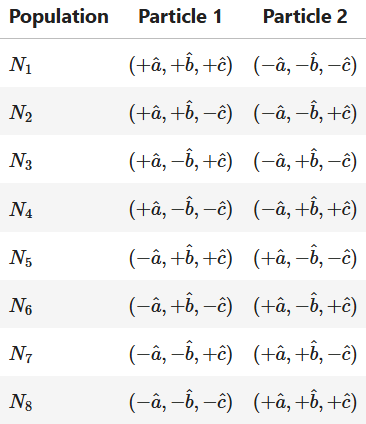
\includegraphics[width=0.5\linewidth]{img/BellList.png}
    \caption{Bell zuständen nach der versteckten Variable}
    \label{fig:BellList}
\end{figure}

Jetzt errechnen wir die Wahrscheinlichkeit das Alice und Bob, bei unabhängigen Messungen, das selbe vorzeichen messen. Die Wahrscheinlichkeit in Zeile 1 und 8 sind $0\%$und in Zeile 2 bis 7 sind es $P = \frac{4}{9}$.
Das bedeutet das nach Einstein die Wahrscheinlichkeit das Alice und Bob das selbe messen $P \leq \frac{4}{9}$ ist. Dies ist Bell`s Inequalität.\\
Vorliegendes beispiel ist generalisiert und kann auf beliebige Winkel angewendet werden, wobei die Wahrscheinlichkeit wie folgt für alle möglichen Winkel berechnet wird.
\begin{equation}
    E(\overrightarrow{a}, \overrightarrow{b}) = \int d\lambda \rho(\lambda) A(\overrightarrow{a}, \lambda) B(\overrightarrow{b}, \lambda)
\end{equation}

Nun zu der Wahrscheinlichkeit nach der Quantenmechanik. Wir gehen davon aus das Bob den spin in $a$ richtung misst beispielsweise spin up, daraus folgernd muss wenn Alice in $a$ richtung misst das Ergebniss spin down sein.\\
Dadurch das wir das Ergebniss einer der achsen kennen, können wir die Wahrscheinlichkeit für die anderen Achsen mit folgender Gleichung berechnen.
\begin{equation}
    P(b) = \cos^2(\frac{\theta}{2})
\end{equation}
Hierbei ist $\theta$ der Winkel zwischen den Achsen. Wenden wir dies auf das beispiel auf die Achse $b$ an so setzen wir $\theta = 60^\circ$
\begin{equation}
    P(b) = \cos^2(\frac{60^\circ}{2}) = \frac{3}{4}
\end{equation}
Machen wir dies auch für die andere Achse $c$ wo $\theta = 120^\circ$ ist erhalten wir
\begin{equation}
    P(c) = \cos^2(\frac{120^\circ}{2}) = \frac{1}{4}
\end{equation}
Von diesen beiden Wahrscheinlichkeit errechnen wir den durchschnitt von $P = \frac{1}{2}$, was bedeutet das Bell`s Inequalität mit $P = \frac{1}{2} \ge \frac{4}{9}$ verletzt ist.\\

\subsubsection{Bell im Quantumcomputer}
\label{subsubsec:bell_quantumcomputer}
Wir haben das Beispiel von Bell`s Inequalität in der Quantenmechanik gezeigt, jedoch ist es auch möglich dies in einem Quantumcomputer zu zeigen.
Hierbei haben wir das Bells Theorem folgendermaßen umgesetzt.
\begin{figure}[H]
    \centering
    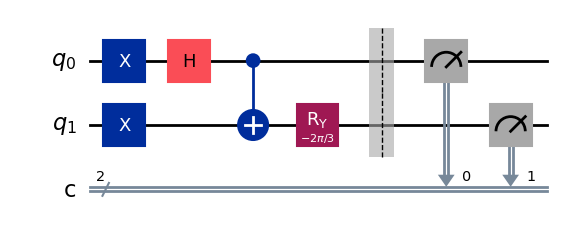
\includegraphics[width=0.9\linewidth]{img/BellCircuit.png}
    \caption{Bell`s Theorem im Quantumcomputer}
    \label{fig:BellCircuit}
\end{figure}

Die beiden linien $q_0$ und $q_1$ sind die beiden verschränkten Teilchen, die durch den zerfall eines Teilchens entstanden sind.
Den verschänkten zustand erreichen wir durch die beiden $X$ gates, dass $H$ gate und das CNOT gate.
Nachdem wir den verschränkten Zustand erreicht haben, messen wir $q_0$ in der $a$ Achse und $q_1$ an der $b$ Achse. Dies ist mit dem $R_y$ gate realisiert der die messung um $120^\circ$ dreht.\\

Um eine genaueres Ergebniss zu erhalten, führen wir diese Messungen 30000 mal durch
\begin{figure}[H]
    \centering
    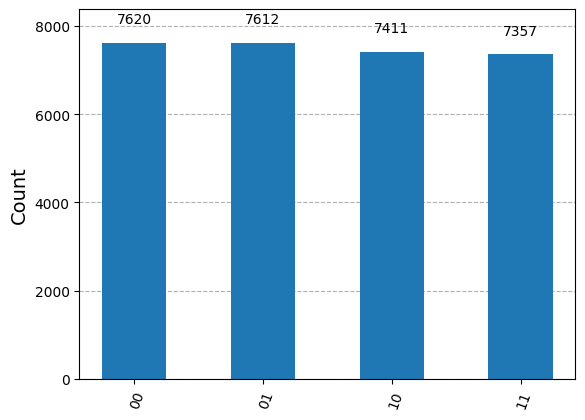
\includegraphics[width=0.8\linewidth]{img/BellResult.png}
    \caption{Ergebniss von Bell`s Theorem im Quantumcomputer}
    \label{fig:BellResult}
\end{figure}

Die Ergebnisse zeigen das die Wahrscheinlichkeit das selbe vorzeichen zu messen bei $P = (7620 + 7357) / 30000 = 0.49923$ oder auch 49,923\% liegt, was Bell`s Inequalität verletzt.\\


\subsection{CHSH experimentell}
\label{subsec:chsh_experimentell}


\subsection{local hidden variable theory}
\label{subsec:chsh_lhvt}